\documentclass[paper=a4,fontsize=9pt]{scrartcl}
\usepackage[english]{babel}
\usepackage{graphicx}
\usepackage[svgnames]{xcolor}
\usepackage{geometry}
\textheight=700pt
\usepackage{url}
\usepackage{fontawesome5}
\usepackage[export]{adjustbox}
\usepackage{sectsty}
\usepackage{hyperref}
\usepackage{amsmath}
\usepackage{enumitem}

\pagestyle{empty}
\sectionfont
{
    \usefont{OT1}{phv}{b}{n}
    \sectionrule{0pt}{0pt}{-5pt}{1pt}
}

%%% Macros
%%% ------------------------------------------------------------
\newlength{\spacebox}
\settowidth{\spacebox}{8888888888}
\newcommand{\sepspace}{\vspace*{1em}}

\newcommand{\MyName}[1]{
        \Huge \usefont{OT1}{phv}{b}{n} \hfill #1
        \par \normalsize \normalfont}
		
\newcommand{\MySlogan}[1]{
		\large \usefont{OT1}{phv}{m}{n}\hfill #1
		\par \normalsize \normalfont}

\newcommand{\NewPart}[1]{\section*{\uppercase{#1}}}

\newcommand{\PersonalEntry}[2]{
		\noindent\hangindent=0em\hangafter=0
		\parbox{\spacebox}{#1}
		\hspace{2.5em} #2 \par}

\newcommand{\SkillsEntry}[4]{
		\noindent \textbf{#1} \hfill
		\colorbox{White}{\color{White}#2} \par
		\noindent #3 \par
		\noindent\hangindent=2em\hangafter=0 \small
        \begin{itemize}[itemsep=0pt, topsep=0pt, leftmargin=1.2em, label={}]
            \item #4
        \end{itemize}
		\normalsize \par}

\newcommand{\ExperienceEntry}[4]{
	\noindent \textbf{#1} \hfill
	\colorbox{Grey}{
		\parbox{6em}{
		\hfill\color{White}#2}} \par
	\noindent #3 \par
    \noindent \small #4
	\normalsize \par
}

%%% ------------------------------------------------------------
\begin{document}

\noindent
\begin{minipage}[t]{3.8cm}
    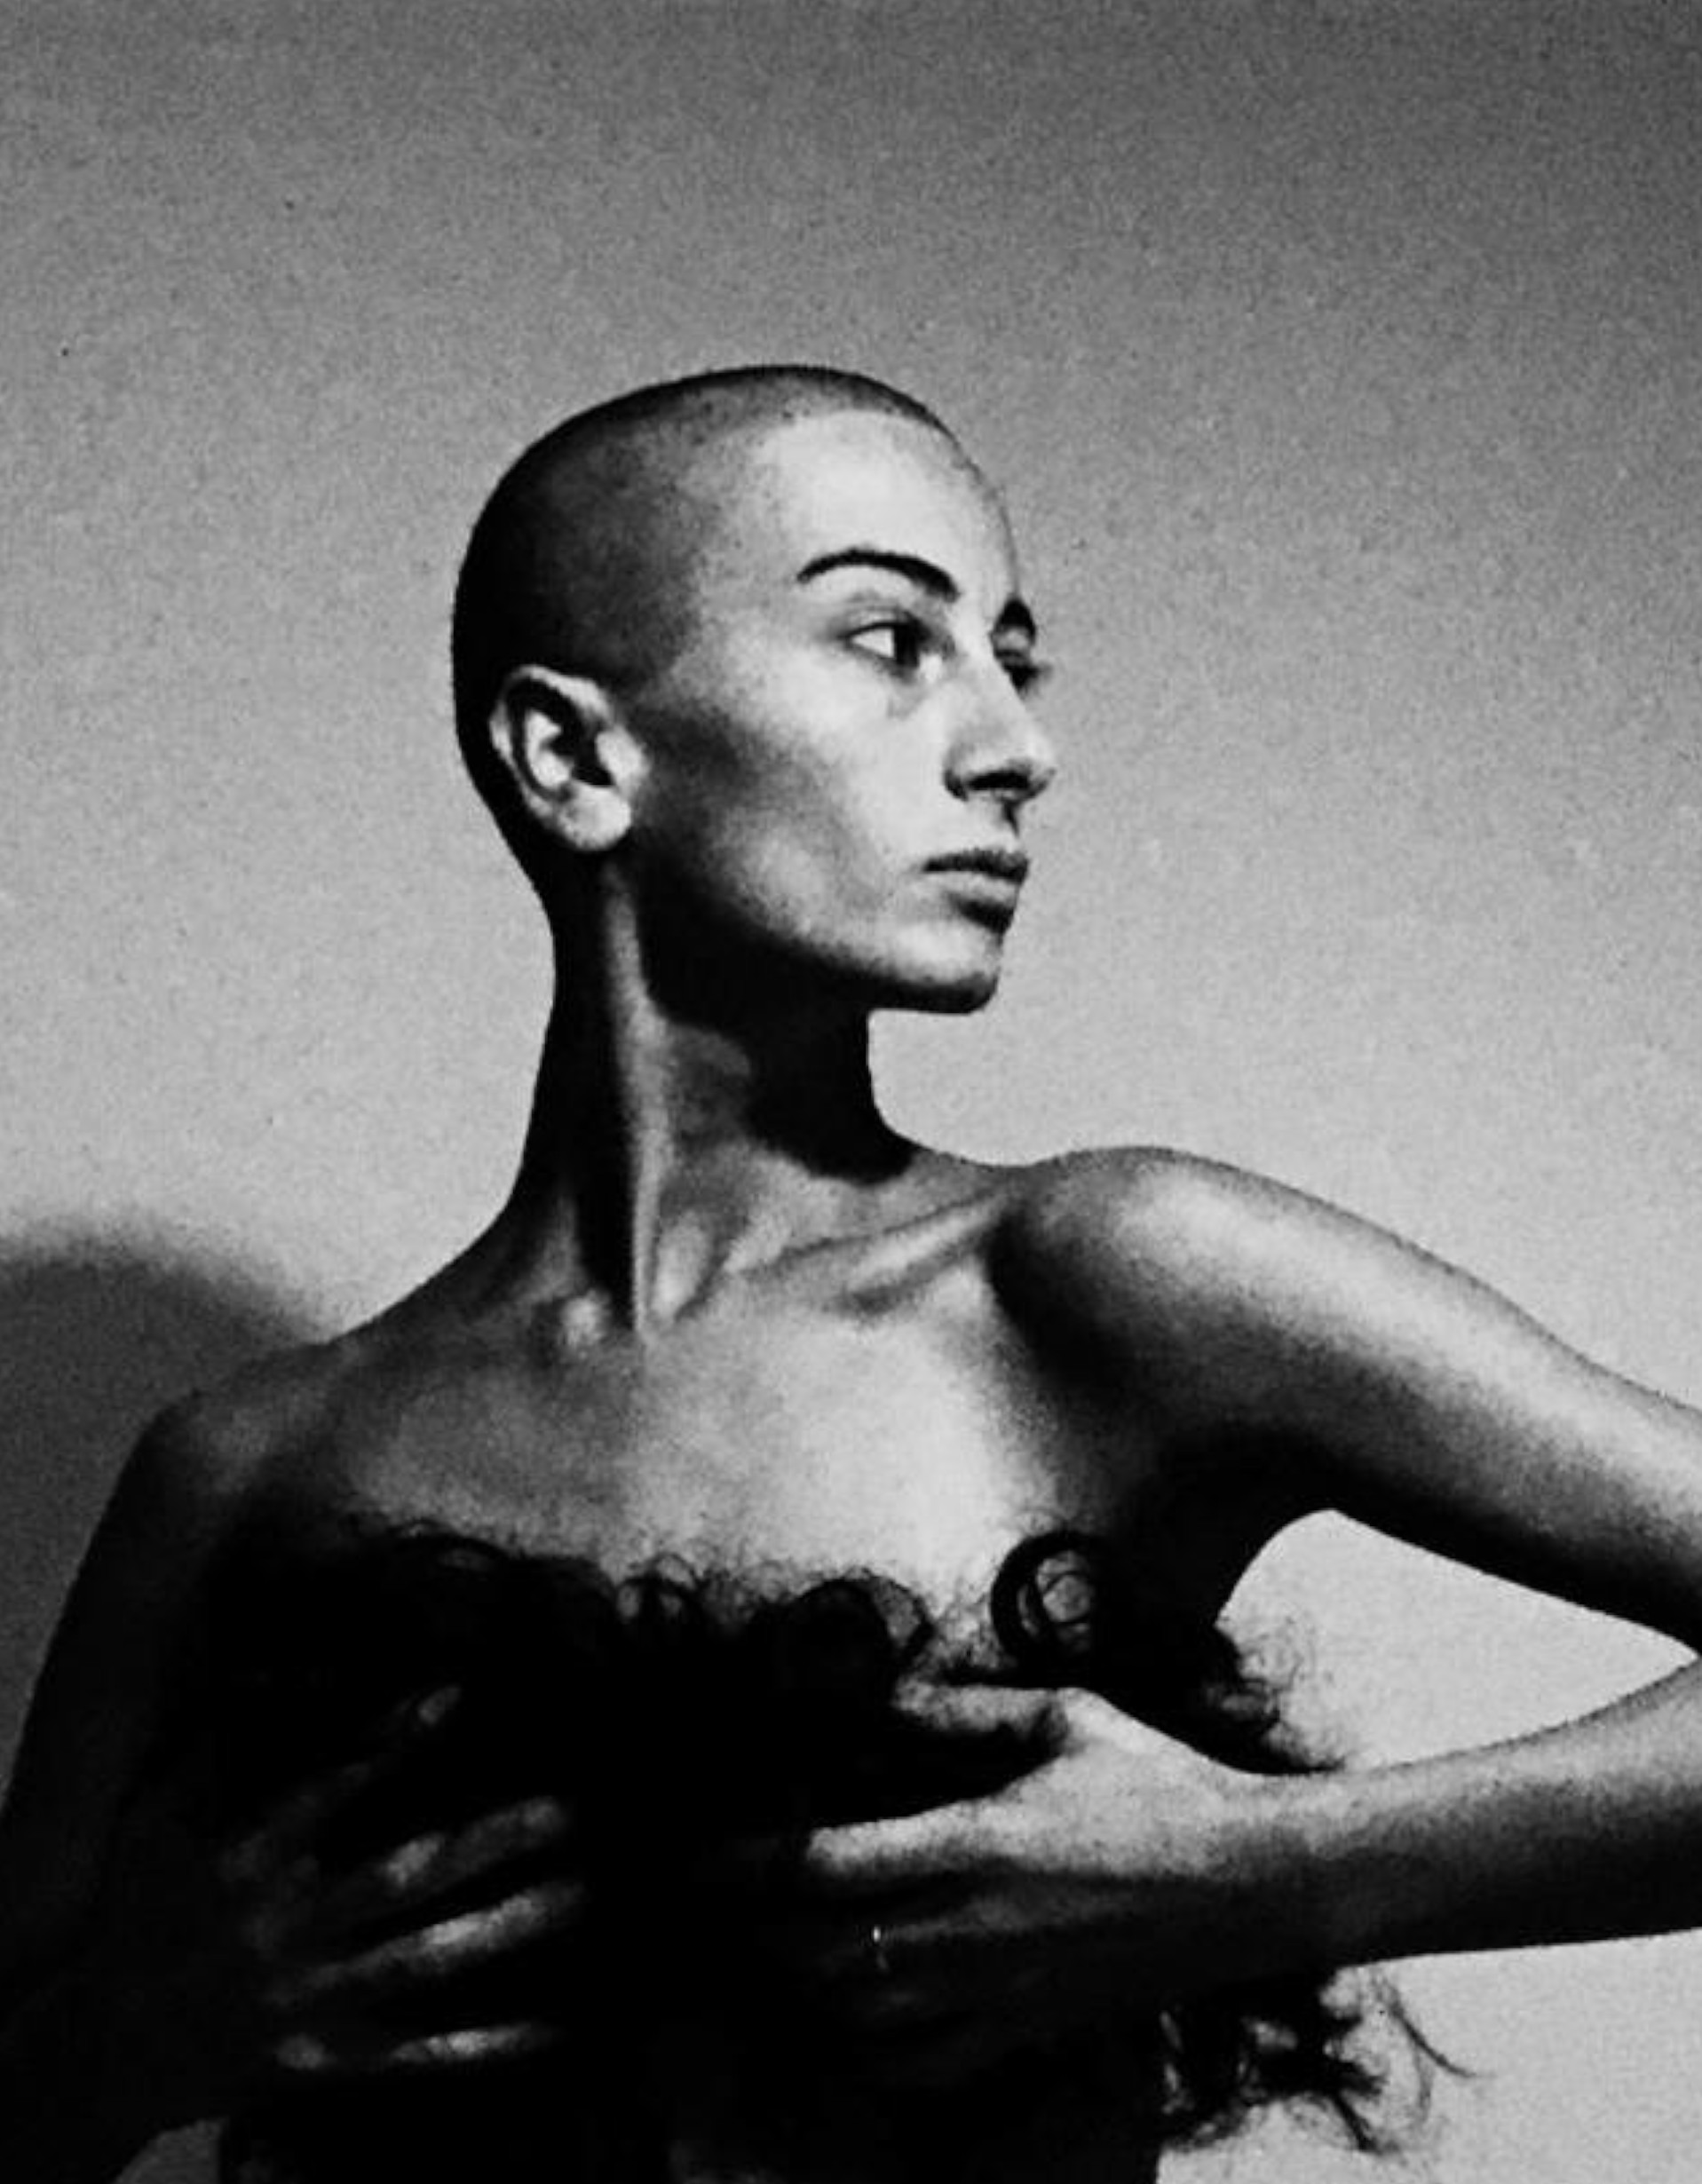
\includegraphics[height=4cm, valign=t]{images/portrait}
\end{minipage}
\hspace{1em}
\begin{minipage}[t]{0.7\textwidth}
    \MyName{Simon Zimmermann}
    \MySlogan{Software Developer}
    \sepspace
    \sepspace
    \sepspace
    \sepspace
    \sepspace
    \PersonalEntry{Birth}{June 5, 1993}
    \PersonalEntry{Location}{Düsseldorf, Germany}
    \PersonalEntry{Mail}{\url{mail@simonzimmermann.com}}
    \PersonalEntry{Github}{\faGithub\space\url{github.com/SimonZimmer}}
\end{minipage}

%%% ------------------------------------------------------------
\NewPart{Work Experience}{}
\ExperienceEntry{Dear Reality GmbH}{2022-present}{C/C++ Backend Software Developer}{
    \begin{itemize}[itemsep=0pt, topsep=1pt, leftmargin=1.2em]
        \item Designed proprietary C-API based on DSP-prototypes using C99, C++17.
        \item Applied DSP-research in prototypes for internal evaluation using Python and MATLAB.
        \item Researched new developments in Digital Signal Processing related to Spatial audio.
        \item Developed custom API-wrapping tooling to facilitate rapid prototyping using C99 and Pure Data (Pd).
        \item Maintained DevOps pipelines using Microsoft Azure for Continuous Integration and Delivery of proprietary APIs and internal packages.
    \end{itemize}
}
\sepspace
\ExperienceEntry{Dear Reality GmbH}{2020-2022}{C++ Fullstack Software Developer}{
    \begin{itemize}[itemsep=0pt, topsep=1pt, leftmargin=1.2em]
        \item Full-stack development of real-time audio applications following test-driven development, modern C++ and agile project management principles.
        \item Designed cross-platform file codecs and internal tooling for maintaining data updates using FlatBuffers, Python, and Docker.
        \item Implemented Google Analytics and license-management for audio plugins
        \item Maintained self-hosted Jenkins build pipeline for Continuous Integration and Delivery.
    \end{itemize}
}
\sepspace
\ExperienceEntry{Dear Reality GmbH}{2017-2020}{Researcher/QA Engineer}{
    \begin{itemize}[itemsep=0pt, topsep=1pt, leftmargin=1.2em]
        \item Full-stack development of real-time audio applications following test-driven development, modern C++ and agile project management principles.
        \item Developed framework for automated real-time audio plugin testing.
        \item Developed DSP prototypes related to spatial audio.
        \item Tested real-time audio tools for quality assurance.
    \end{itemize}
}
\sepspace
\ExperienceEntry{ISRW-Klapdor}{2016-2017}{Room-Acoustics Engineer}{
    \begin{itemize}[itemsep=0pt, topsep=1pt, leftmargin=1.2em]
        \item Predictive simulation of room properties during construction to meet regulatory needs for speech intelligibility and thermal insulation in buildings.
        \item In-situ measurement and evaluation of room-acoustic properties during construction.
    \end{itemize}
}

%%% ------------------------------------------------------------
\NewPart{Projects}{}
\ExperienceEntry{dearVR Exoverb}{2022}{C/C++ Developer}{
    \begin{itemize}[leftmargin=1.2em, label={}]
        \item Developed Reverb plugin with enhanced spatial perception that simulates acoustic scenes with three-dimensional depth and width using synthesized spatial room impulse responses.
    \end{itemize}
}
\sepspace
\ExperienceEntry{Team Split Facilitation}{2022}{C/C++ Developer, DevOps Engineer}{
    \begin{itemize}[leftmargin=1.2em, label={}]
        \item Transition from a single-team full-stack workflow to a frontend/backend team split with modernized DevOps infrastructure for continuous integration from an on-premise solution to a cloud-based solution.
    \end{itemize}
}
\sepspace
\ExperienceEntry{dearVR MIX/MONITOR}{2021}{C++ Full Stack Developer}{
    \begin{itemize}[leftmargin=1.2em, label={}]
        \item Developed the multichannel immersive headphone mixing plugins "dearVR MIX" and "dearVR MONITOR" which utilize headphone calibration, room simulation, and binauralization to virtualize studio environments. Supports adjustable virtual mix rooms and 26 multi-channel loudspeaker formats up to 9.1.6.
    \end{itemize}
}

\NewPart{Publication}{}
\ExperienceEntry{Co-Author}{2021}{Conference Paper}{
    \begin{itemize}[leftmargin=1.2em, label={}]
        \item Immersive and 3D Audio: from Architecture to Automotive (I3DA): "Machine Learning-Based Room Classification for Selecting Binaural Room Impulse Responses in Augmented Reality Applications".
    \end{itemize}
}

%%% ------------------------------------------------------------
\NewPart{Education}{}
\ExperienceEntry{M.Sc. Media Informatics}{2018-2020}{University of Applied Sciences, Düsseldorf}{
    \begin{itemize}[leftmargin=1.2em, label={}]
        \item Thesis title: 'Scalable Modelling of Room Acoustic Characteristics for AR devices on the Basis of Visual Information Using Deep Learning' - honors degree.
    \end{itemize}
}
\sepspace
\ExperienceEntry{M.Sc. Music Informatics}{2018}{University of Music, Karlsruhe}{
    \begin{itemize}[leftmargin=1.2em, label={}]
        \item Guest Semester.
    \end{itemize}
}
\sepspace
\ExperienceEntry{B.Eng. Media Engineering}{2012-2017}{University of Applied Sciences, Düsseldorf}{
    \begin{itemize}[leftmargin=1.2em, label={}]
        \item Thesis title: 'A Concept for Implementing Room Acoustic Properties in the Context of a 3D-Audio Engine'.
    \end{itemize}
}

%%% ------------------------------------------------------------
\NewPart{Skills}{}
\SkillsEntry{Technologies}{}{}{\textsc{C++17}, C99, Boost, CMake, Conan, Python, gtest/gmock, Google Benchmark, Pure Data (Pd), Azure DevOps, Github Actions, Jenkins, Git, Docker, JUCE, pybind11, Flask, Wagtail, MATLAB, \LaTeX, Linux, nvim/vim, Google Analytics}
\sepspace
\SkillsEntry{Languages}{}{}{German (native), English (fluent)}
\sepspace
\SkillsEntry{Other}{}{}{Music Production, Modular Synthesizer, Esoteric Programming Languages (Orca, TidalCycles)}

\end{document}

